%\chapter{Referencial Teórico}
\chapter{Fundamentação Teórica} 
\label{cap:referencial_teorico}

Um veículo autônomo tem como problemática básica as questões referentes ao
mapeamento, localização e navegação, as quais são fortemente influenciadas pelas
características do ambiente, do problema em questão a ser tratado e da
configuração do robô (sensores e atuadores) \cite{Wolf2009}. Quando se trata
de navegação em ambiente externo, o desconhecimento do ambiente e da sua
dinâmica tornam o mapeamento e localização mais críticos. Em um ambiente
semi-estruturado podemos considerar a existência de algum referencial e impor
alguma restrição, como a existência de caminhos bem definidos e guias, porém
estes devem ser considerados intermitentes, ou seja, o sistema deve ser mais
tolerante à perda momentânea de referenciais. Quando o ambiente não é
estruturado depara-se com a falta de referenciais elementares (linhas, paredes,
trilhas ou vias de deslocamento bem definidas) e com a baixa possibilidade de
imposição de restrições. O desenvolvimento de um sistema autônomo para um
veículo móvel se caracteriza primariamente pelo tratamento destas questões. 

%2012-10-14 Lido OK


%Revisar paragrafo
As pesquisas em veículos terrestres autônomos têm crescido nos últimos anos e já
apresentam aplicações práticas principalmente pela indústria automobilística
para uso em ambiente urbano para o aumento da segurança no uso de automóveis e
na redução de acidentes. Os desenvolvimentos mais recentes podem ser vistos em
\cite{concepts}. 

%Também, a aplicação de veículos terrestres em ambientes
%semi-estruturados ou não estruturados tem chamado a atenção. Este tipo de
%aplicação tem grande interesse econômico em aplicações agrícolas, por exemplo.

Por outro lado, a aplicação de veículos terrestres autônomos em ambientes
semi-estruturados e não estruturados tem também chamado a atenção. Um exemplo
deste tipo deste tipo de utilização são os veículos adotados em aplicações
agrícolas, como já foi citado. 


\section{Mapeamento e Localização}
\label{sec:mapeamento_localizacao}

%A questão do mapeamento e localização é considerado um problema central na
%robótica móvel, 

O mapeamento e localização é uma necessidade recorrente nas aplicações em
robótica móvel, onde a caracterização do veículo como autônomo de fato pode vir
a ser dada essencialmente pela sua capacidade de tratar esta questão. Para que
um robô possa ir de um ponto ao outro do ambiente ele deve conhecer, pelo menos,
a sua localização e a localização do seu ponto de destino. Quando o mapa e a
estrutura do ambiente, assim como a localização do veículo, são desconhecidos a
priori essa questão se torna crítica. Esta necessidade é denominado de SLAM
(\textit{Simultaneous Localization and Mapping}) e é um problema central na
robótica móvel, onde ambas informações dependem uma da outra para serem obtidas. Um
algoritmo proposto para solucionar o SLAM é apresentado em \cite{Thrun2004} que
utiliza uma abordagem probabilística onde as estimativas tando da posição como
do mapeamento são atualizadas uma a partir da outra a medida que dados
sensoriais são coletados.

A visão computacional tem sido aplicada em soluções para o tratamento de SLAM
como a fonte de informação sensorial. Outros equipamentos, como sensor a laser
utilizado em \\\cite{Lategahn2011} e até mesmo sensores inerciais (IMU -
\textit{Inertial Measurement Unit}), como apresentado em \cite{FootSLAM}, são
aplicados e combinados com o propósito de aumentar a acurácia destas medições.
% a localização é estimada pelo onde o erro da estimativa da localização reduz a
% medida que o mapeamento Esse problema é normalmente tratado através de
% abordagens como o SLAM (\textit{Simultaneous Location and Mapping}).
% Uma solução robusta e eficiente para a questão de localização e mapeamento
% simultâneos (SLAM) na prática ainda é desafiadora (\cite{Dissanayake2001}) A
% visão computacional tem sido aplicada em soluções para o tratamento de SLAM ,
% onde uma abordagem recorrente no tratamento da localização e do mapeamento é a
% utilização de visão computacional.
% Porém há uma diversidade de sensores que podem ser integrados com o propósito
% de aumentar a acurácia destas medições, trabalhos recentes como o de
% \cite{FootSLAM} apresenta uma abordagem baseada em sensores inerciais (IMU -
% \textit{Inertial Measurement Unit}).
Entretanto, em ambientes externos (\textit{outdoor}) e extensos a construção de
um mapa global a partir dos dados sensoriais pode não ser viável, comprometendo
a estimação da localização baseada em mapa.
% e a definição da localização em relação a este mapa pode se tornar um problema
% intratável .
Uma solução para determinação da localização em ambientes externos é a obtenção
de coordenadas através do uso do GPS (\textit{Global Positioning System}), que é
baseado na trilateração das distâncias do veículo em relação a uma “constelação”
de satélites deste sistema. Portanto, a posição do veículo e de seu destino pode
ser estimada diretamente (com um certo erro) a partir das informações fornecidas
por um aparelho localizador GPS.



%OSORIO
%> Podia discutir um pouco mais sobre estas questões (expandir esta seção):
%- Dependência da existência de um mapa previamente definido (mapeado pelo robô
%ou não) e do planejamento prévio da rota do robô, ou, navegar no ambiente
%(usualmente não estruturado) sem o uso de um mapa ou de um planejamento prévio
%de rotas (existe o risco de ficar bloqueado, pois possui apenas o conhecimento
%local do ambiente e não realiza um plano global => é bom mostrar que está
%consciente disto).
%- Dependência de um mapa (global) exato e de uma localização exata, ou
%alternativamente, usa um mapa aproximado (local) e usa uma localização também
%aproximada (não muito precisa).
%> São abordagens possíveis e podemos "escolher" entre elas de acordo com o
%problema e requisitos impostos pela aplicação. Obviamente neste trabalho foi
%feita uma escolha (e espero que o leitor se convença que foi uma boa escolha
%dado o contexto)    :)


A localização pode se beneficiar quando há mapas previamente fornecidos, sendo
necessária a localização da posição inicial em relação ao mapa. Os mapas têm
papel importante na tarefa de navegação (seção \ref{sec:navegacao}), tanto
quando fornecidos previamente como quando construídos no momento em que o
veículo se desloca no ambiente. O mapa para navegação geralmente se caracteriza como
local ou global \cite{concepts}. O mapa global provê informações mais
abrangentes sobre o espaço onde o veículo irá se deslocar, principalmente
fornecendo informações sobre obstáculos estáticos e zonas navegáveis
preferenciais, como estradas. Estas informações dos mapas normalmente se
associam a custos, os quais são utilizados pelos algoritmos de planejamento
buscar o melhor caminho. Também, os mapas podem ser representados de forma
métrica (geométrica) e/ou topológica - contendo informações mais detalhadas de o
quê ocupa um determinado espaço (prédio, vegetação, etc.)\cite{Thrun98a}. Já os
mapas locais têm o papel de expressar o ambiente dentro do raio de atuação dos
sensores, ou seja, uma noção localizada próxima ao veículo. Estes mapa local
contém a visão mais atual do ambiente, contemplando obstáculos dinâmicos. A
construção do mapa local pode ser utilizado para agregar informações e atualizar
o mapa global, desta forma, o mapa global se traduz em uma memória do espaço
para o veículo (\fig{fig:map2d}). Quando não há informação prévia que possa ser
utilizada como mapa global é usual uma navegação prévia para o reconhecimento do
ambiente antes que se efetuem tarefas específicas de navegação. Este
reconhecimento inicial pode ser feito de forma autônoma apenas vagando no
ambiente como uma navegação guiada.

\begin{figure}[ht]
%	\centering
	\begin{minipage}[b]{0.9\linewidth}
	    \centering
	    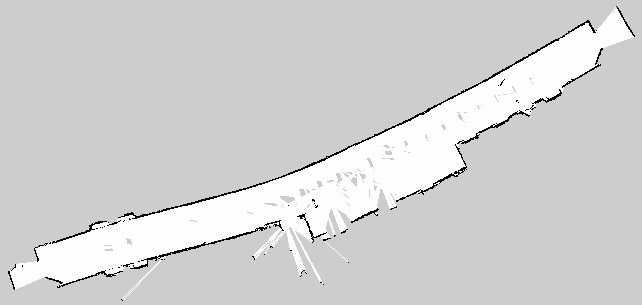
\includegraphics[width=\textwidth,height=6cm]{images/map_2d.jpg}
	 	\caption{Mapa de ocupação planar: Em branco o espaço live, em preto o espaço
	 	ocupado e em cinza o espaço sem informação de ocupação}
		\fonte{www.ros.org (divulgação)}
	 	\label{fig:map2d}
	\end{minipage}
\end{figure}

%2012-10-15 Lido OK (pode ainda ser mais desenvolvido)


\section{Informação Sensorial: Visão Computacional}

Um veículo móvel terrestre se desloca (geometricamente) apoiado sobre um plano
de suporte, ou seja, seus graus de liberdade usualmente podem ser considerados
em duas dimensões. Desta forma, o reconhecimento do chão representa uma
necessidade e se caracteriza um importante desafio ao se considerar um ambiente
externo não estruturado composto por um solo com vegetação. Além da detecção do
chão, é necessária uma certa classificação das regiões deste plano de suporte
(solo) como sendo, por exemplo, uma superfície transitável ou não transitável:
devido à presença de vegetação, obstáculos, buracos e demais impedimentos.
Os sensores típicos, como sonares e lasers, não apresentam dados muito adequados
para viabilizar essa classificação, uma vez que o sonar possui uma limitação de
alcance e de precisão e o sensor laser de 1 feixe é capaz apenas de analisar uma
seção planar do espaço tridimensional (além de ter um custo muito elevado para
certas aplicações). As câmeras de vídeo são mais adequadas para capturar tais
informações que caracterizam o ambiente, principalmente, se forem usadas câmeras
estéreo, das quais é possível extrair uma informação de profundidade dos
elementos da cena capturada. A utilização de câmeras de vídeo demandam algumas
tarefas elementares, como o ajuste de foco, a utilização de lentes adequadas ao
ângulo de visão necessário e uma devida calibragem. A calibragem das câmeras é
um processo fundamental para se obter um sistema de visão computacional com
representação tridimensional a partir de um par de câmeras independentes
(binocular). Neste processo são calculados (estimados) os parâmetros internos e
externos de cada câmera. Estes parâmetros são essenciais para a reconstrução
tridimensional a partir das imagens capturadas pela câmera estéreo
\cite{Faugeras1993}.

A estimação dos parâmetros internos (intrínsecos) consiste em se obter a
distância focal e o ponto central da imagem, que por questões de alinhamento
entre lentes e sensor pode não ser o pixel central da imagem, influenciando
fortemente os demais processos de estimação \cite{WilsonShafer1994}. Estes
dois parâmetros definem como a imagem é formada por uma câmera estilo
estenopeica (\textit{pin-hole}) e a sua projeção perspectiva. Outros parâmetros
também internos, não associados com o modelo de projeção e sim com as
características físicas das lentes utilizadas, também são estimados no processo
de calibragem. No caso das câmeras de vídeo existe a necessidade de utilização
de lentes, tanto para reduzir a imagem a ser projetada no sensor (filme/CCD)
como para aproximá-las. As lentes comumente são estruturas com curvatura
esférica, característica esta que provoca distorções óticas na imagem projetada.
Estes efeitos são chamados de distorções radiais, produzindo imagens com
demonstrado na \fig{fig:distortions}, nos casos, onde esta distorção pode ser em
forma de “barril” (\textit{barrel}) ou “almofada” (\textit{pincushion})
\cite{Weng1992}.

% (\fig{fig:int_param}).
As distorções óticas influenciam fortemente de forma negativa o processo de
correspondência entre as imagens para extrair a informação tridimensional, sendo
grande fonte de ruído quando não corrigidas. É interessante notar que,
matematicamente, o processo de correção das distorções óticas se baseia na
curvatura esférica da lente, porém as lentes são formadas por uma composição de
várias camadas com curvaturas diferentes (\fig{fig:lens}), que ainda podem
apresentar defeitos no processo de fabricação. Portanto, o modelo matemático
utilizado na correção é sempre uma aproximação global do aparato ótico, fonte
por si só de imprecisão \cite{WilsonShafer1994}.

%Existem ainda outros
%parâmetros que podem ser considerados, porém, estes estão associados a questões
%técnicas da forma de aquisição da imagem e não à formação da imagem propriamente
%dita, portanto são subjetivas ao aparato utilizado sendo necessárias ou não, a
%exemplo, os problemas referentes ao entrelaçamento e varredura da imagem.

% \begin{figure}[ht]
% 	\centering
% 	\begin{minipage}[b]{0.3\linewidth}
% 	    \centering
% 	    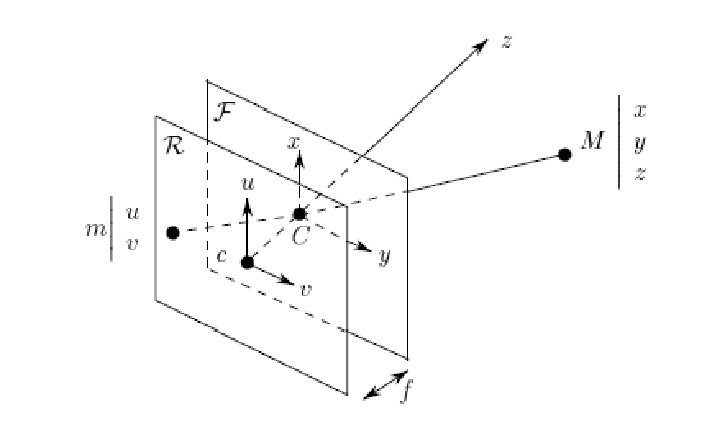
\includegraphics[width=\textwidth]{images/int_param.png}
% 	 	\caption{Ponto central e distância focal}
% 		\fonte{(\cite{Faugeras1993})}
% 	 	\label{fig:int_param}
% 	\end{minipage}
% 	\hspace{0.1cm}
% 	\begin{minipage}[b]{0.3\linewidth}
% 	    \centering
% 	    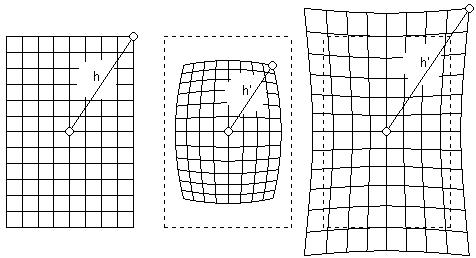
\includegraphics[width=\textwidth]{images/distortions.png}
% 	 	\caption{Distorções óticas}
% 	 	\label{fig:distortions}
% 	\end{minipage}
% 	\hspace{0.1cm}
% 	\begin{minipage}[b]{0.3\linewidth}
% 		\centering
% 	    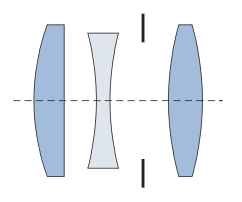
\includegraphics[width=\textwidth,height=3cm]{images/lens.png}
% 	 	\caption{Exemplo de composição ótica}
% 	 	\label{fig:lens}
% 	\end{minipage}
% \end{figure}

\begin{figure}[ht]
	\centering
	\hspace{0.1cm}
	\begin{minipage}[b]{0.45\linewidth}
	    \centering
	    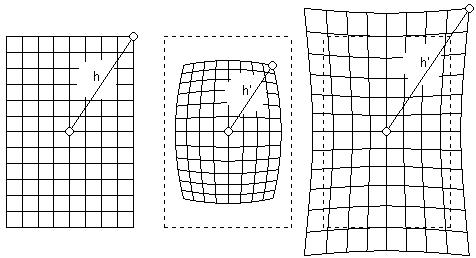
\includegraphics[width=\textwidth]{images/distortions.png}
	 	\caption{Distorções óticas: sem distorção (\textit{esquerda}), 
	 	distorção tipo “barril” (\textif{centro}), 
	 	distorção tipo “almofada” (\textit{direita}).}
	 	\label{fig:distortions}
	\end{minipage}
	\hspace{0.1cm}
	\begin{minipage}[b]{0.45\linewidth}
		\centering
	    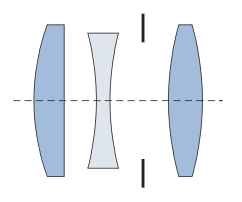
\includegraphics[width=\textwidth,height=4cm]{images/lens.png}
	 	\caption{Exemplo de composição ótica de lentes.}
	 	\label{fig:lens}
	\end{minipage}
\end{figure}


De posse dos parâmetros internos associados às distorções é necessário um
pré-processamento para a sua correção que ao ser aplicado produz uma imagem mais
própria para os algoritmos de correspondência que formarão a imagem
tridimensional. Os parâmetros internos são também chamados de parâmetros do
modelo, isto é, como a imagem é formada. Um outro modelo de câmera geralmente
associado a veículos móveis são as câmeras omnidirecionais, capazes de produzir
uma imagem em 360 graus, útil para veículos com esse grau de liberdade de
movimentos. A calibragem deste tipo de câmera é ainda mais complexa. O segundo
conjunto de parâmetros são os parâmetros externos (extrínsecos), também chamados
de parâmetros de pose. Este conjunto diz respeito à posição da câmera em relação
ao ambiente, no caso, a um sistema de coordenadas referencial. Estes são os
principais parâmetros para a reconstrução tridimensional, pois são utilizados
para se chegar a uma correspondência entre os pixeis de cada uma das duas
imagens. Esta correspondência entre os pontos é obtida pelos princípios da
geometria epipolar (\fig{fig:epipolar}) \cite{Faugeras1993}. De posse dessa
correspondência, a partir do deslocamento destes pontos (disparidade) e um
processo de triangulação, pode ser construída uma representação tridimensional
em um mapa de profundidade. Fundamentalmente, são determinados os planos
formados pelos pontos em comum em cada imagem (referenciais obtidos pela
calibragem) e o ponto central de cada imagem. Esses planos no espaço (ambiente)
são coincidentes, ou seja, o mesmo plano de corte. Esta projeção do plano em
cada imagem definem retas, chamadas retas epipolares. Desta forma é possível
fazer a correspondência dos demais pontos (não referenciais). Este alinhamento
das imagens é chamado de retificação \cite{Fusiello2000}, como pode ser visto
na \fig{fig:rectification}. Pela geometria epipolar todos os planos formados
pelos pontos referenciais serão concorrentes e as suas intersecções se dão em
uma reta em comum, chamada linha base. Esta linha base determina o alcance da
visão (profundidade).

Em um estudo anterior realizado por Klaser \cite{Klaser2007}, em seu trabalho
de conclusão de graduação (TCC), foi aplicada visão tridimensional para
monitorar experimentos de laboratório utilizando como processo de calibragem o
método de Tsai \cite{Tsai1987}. Naquele trabalho, onde as duas câmeras podiam
ser posicionadas em relação ao ambiente com uma certa liberdade observando-se
alguns critérios, foi possível verificar que um conjunto de referenciais capazes
de descrever os três planos ortogonais do espaço tridimensional produziam uma
calibragem bastante precisa. Para isso, foi utilizado um molde semelhante ao
canto de uma sala contendo pelo menos três pontos referenciais em cada parede e
no chão (\fig{fig:bioview}). Uma vantagem do método de Tsai é que o referencial
para a calibragem é dado informando sua posição na imagem e sua posição real no
ambiente, sendo a posição real dada de forma relativa a um sistema de
coordenadas referencial no espaço. Com isso, ao extrair a informação
tridimensional de um ponto pelo processo de triangulação a partir da calibragem
do par estéreo, a informação resultante contém as coordenadas espaciais do ponto
na unidade de medida adotada. Desta forma, é possível saber a posição real de um
determinado ponto, podendo ser extraída uma nuvem de pontos 3D do ambiente
(\textit{3D point cloud}). Porém, para se obter as coordenadas tridimensionais
de um determinado ponto no espaço é necessário saber onde esse ponto se encontra
em cada imagem \cite{MundyZisserman1994}.
Isto não é trivial, mas é possível utilizar métodos de detecção e casamento
(\textit{matching}) de características (\textit{features}) das imagens para
buscar a correspondência, como por exemplo, o método SIFT
(\textit{Scale-Invariant Feature Transform}) \cite{Lowe1999} e o método SURF
(\textit{Speeded Up Robust Features}) \cite{Bay2008}.
% Uma abordagem baseada neste princípio em que, a partir de duas poses da mesma
% cena, se extrai uma terceira coordenada tendo por base uma calibragem das
% câmeras e um processo de correlação global dos pixeis, é chamada de mapa de
% disparidade. Este processo é computacionalmente custoso e existem diversas
% técnicas para a sua implementação.
Uma abordagem para extrair a terceira coordenada espacial tendo por base duas
imagens da mesma cena em poses diferentes e a devida calibragem é chamada de
disparidade \cite{Qian97binoculardisparity}. Este processo é computacionalmente
custoso e existem diversas técnicas para a sua implementação.

\begin{figure}[ht]
	\begin{minipage}[b]{0.3\linewidth}
	    \centering
	    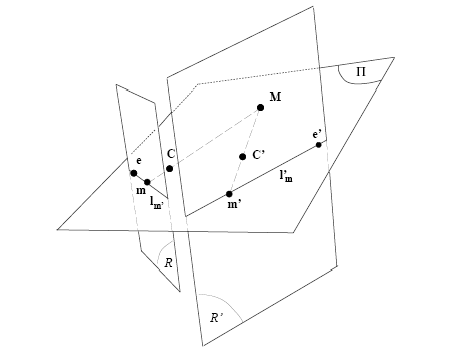
\includegraphics[width=\textwidth]{images/epipolar.png}
	 	\caption{Geometria epipolar}
		\fonte{\cite{Faugeras1993}}
	 	\label{fig:epipolar}
	\end{minipage}
	\hspace{0.1cm}
	\begin{minipage}[b]{0.3\linewidth}
	    \centering
	    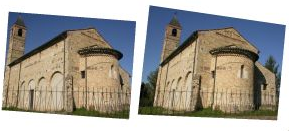
\includegraphics[width=\textwidth,height=4cm]{images/rectification.png}
	 	\caption{Retificação }
		\fonte{Andrea Fusiello}
	 	\label{fig:rectification}
	\end{minipage}
	\hspace{0.1cm}
	\begin{minipage}[b]{0.3\linewidth}
		\centering
	    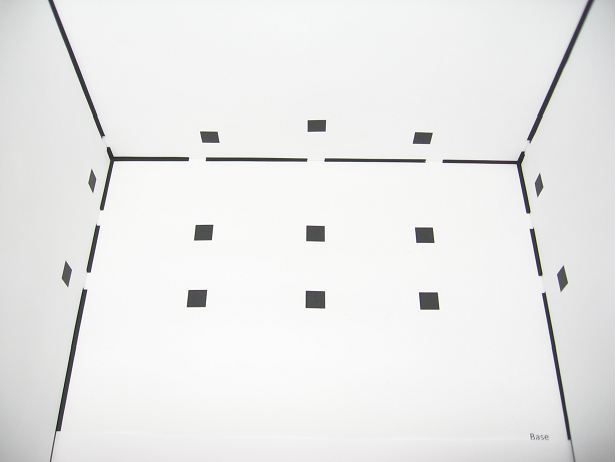
\includegraphics[width=\textwidth,height=4cm]{images/bioview.png}
	 	\caption{Calibragem com referenciais fixos}
		\fonte{\cite{Klaser2007}}
	 	\label{fig:bioview}
	\end{minipage}
\end{figure}

\vspace{0.5cm}


%OSORIO
%> Podia acrescentar uma breve seção sobre GPS:
%2.3 Sensores: Localização e Orientação
%descrevendo sobre a posição (GPS) e orientação (bússola), do veículo e de seu
% destino.
%> O parágrafo abaixo já é uma espécie de "resumo e consolidação" do que foi
%apresentado nas seções anteriores.

Portanto, neste trabalho serão adotados os sensores do tipo GPS e Bússola
(posição e orientação) para localização e câmeras estéreo para a extração de
mapas locais. Estes mapas descreverão o ambiente e os obstáculos através de uma
representação espacial (3D) na qual se encontra o veículo robótico autônomo. A
câmera estéreo irá fornecer um mapa de navegabilidade local composto por
informações obtidas a partir do mapa de disparidade que será descrito a seguir.

%OSORIO
%> Senti falta de uma noção mais geral sobre como passamos da parte de visão
% computacional estéreo para os mapas locais (mapa 3D - cloud of points, mapa local, mapa de navegabilidade). 
% Mapa de disparidade já entra em um conceito específico...
%> Talvez pudesse ter citado o trabalho do Caio (mestrado) e do Patrick
% (mestrado) que tem bons exemplos de mapas (com figuras)  :)


% 2012-10-13 lido OK


\section{Mapas de Disparidade}
\label{sec:mapas_disparidade}

Os mapas de disparidade se tornaram uma ferramenta bastante utilizada para a
percepção tridimensional. Para robôs móveis autônomos os mapas de disparidade
são muito úteis, principalmente na detecção e desvio de obstáculos. O veículo
pode extrair uma informação de profundidade que servirá como parâmetro para a
navegação, por exemplo, uma região frontal de maior profundidade pode
representar um caminho sem obstáculos, livre de objetos e elementos localizados
em frente a câmera. Atualmente, a implementação direta em hardware dos
algoritmos de cálculo do mapa de disparidade a partir de um par de imagens
(câmera estéreo) permite a aplicação em tempo real e de forma embarcada
(\fig{fig:stoc_on_chip}) \cite{Khaleghi2008}.

A ideia fundamental do mapa de disparidade é fornecer uma informação de
profundidade relativa, mapeada diretamente na imagem bidimensional a partir do
valor do pixel. Usualmente são utilizadas imagens em tons de cinza (8
\textit{bits}), fornecendo então até 255 níveis de profundidade. Na
\fig{fig:tsukuba}, o mapa de disparidade está representando os obstáculos mais
próximos por tons mais claros e os obstáculos mais distantes por tons mais
escuros. Desta forma, os pixeis da imagem passam a representar no lugar da
informação de cor ou luminosidade uma informação de profundidade sobre os
elementos da cena. Os dispositivos sensores que fornecem uma imagem colorida
juntamente com o mapa de disparidade têm sido denominados de dispositivos RGB-D
(Imagem RGB + \textit{Depth}/mapa de disparidade). O sensor Kinect da
Microsoft\foot{Microsoft Kinect - http://www.xbox.com/en-us/kinect} fornece
imagens RGB-D com uma precisão de 2047 níveis de profundidade. Uma avaliação da
qualidade do mapa de disparidade produzido pelo Kinect \cite{Khoshelham2012}
mostrou que a relação entre o nível de profundidade e distância não é linear,
onde a distância real dos objetos é gradualmente maior do que a distância
estimada a medida que se afastam da câmera. O Kinect é utilizado atualmente como
base de comparação pois é uma aplicação em larga escala comercial desta técnica
e produz resultados práticos satisfatórios.

\vspace{0.5cm}
\begin{figure}[h!!!]
	\centering
	\begin{minipage}[b]{0.4\linewidth}
	    \centering
	    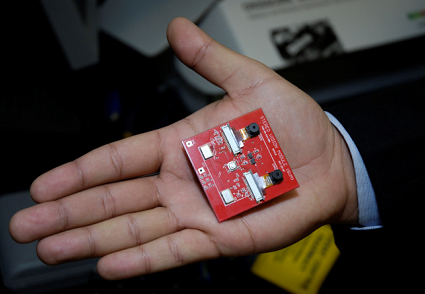
\includegraphics[width=\textwidth,height=4.5cm]{images/stoc_on_chip.png}
	 	\caption{Sistema de visão tridimensional
embarcado baseado em mapa de disparidade}
		\fonte{\cite{Khaleghi2008}}
	 	\label{fig:stoc_on_chip}
	\end{minipage}
	\hspace{0.1cm}
	\begin{minipage}[b]{0.55\linewidth}
	    \centering
	 	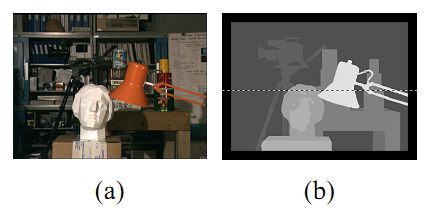
\includegraphics[width=\textwidth,height=4.5cm]{images/tsukuba.png}
	 	\caption{Estéreo: \textbf{(a)} imagem RGB \\ \textbf{(b)} disparidade referencial}
		\fonte{University of Tsukuba}
	 	\label{fig:tsukuba}
	\end{minipage}
\end{figure}

%Porém, essa não linearidade não é um artefato
%que resulta propriamente daquela implementação, 
%ela advém do fato de o mapa ser
%gerado a partir de imagens que são formadas pela projeção perspectiva que 
%inerentemente produz esse efeito (\textit{foreshortening}).

Em sistemas onde as câmeras são estacionárias (fixas em um local), como na
aplicação tradicional do Kinect, técnicas de extração e supressão do fundo podem
ser utilizadas para aumentar a robustez do método \cite{Ivanov2000}. No caso das
aplicações em robótica móvel, as câmeras estão em constante movimento
potencializando estes efeitos negativos, fazendo-se necessário outros métodos
para minimizar estes efeitos. Outra característica a ser apontada em relação ao
Kinect é sua inviabilidade de uso no ambiente externo, ou seja, com iluminação
natural - isto se deve ao fato da tecnologia empregada se basear em luz
estruturada e requer iluminação artificial (infra-vermelho) a qual sofre
interferência na presença de luz solar. Em ambiente externo são utilizadas
câmeras convencionais, onde o conjunto estéreo pode ser constituído tanto por
câmeras independentes permitindo maior versatilidade de poses como no uso de
câmeras do tipo STOC (\textit{STereo On a Chip}) que são mais estáveis em
relação à manutenção da calibragem.

%Em ambiente externo são utilizadas câmeras convencionais
%porém geralmente o uso de câmeras estéreo tipo STOC (\textit{STereo On a Chip})
%são um tipo de aplicação por serem mais estáveis em relação à manutenção da
%calibragem devido a vibrações.

%Fig. 2.7: Sistema de visão tridimensional
%embarcado baseado em mapa de disparidade
%Fonte: 
%Fig. 2.8: a) Imagem RGB; b) Mapa de disparidade Fonte: University of Tsukuba 

O mapa de disparidade provê uma percepção espacial que representa os elementos
da cena em um espaço tridimensional, fornecendo assim, uma fonte muito rica de
informações sobre a cena. A partir destas informações pode ser possível então
definir a trajetória do veículo de modo a desviar dos obstáculos que se
encontram a sua frente ao mesmo tempo em que este se locomove em direção ao seu
destino. Este processo é denominado de navegação robótica e será detalhado a
seguir.


%%2012-10-14 Lido OK

\section{Navegação}
\label{sec:navegacao}

A navegação em campo aberto se torna um problema de tomada de decisões difícil,
devido à ausência de um mapa global atualizado, a falta de referenciais locais e
o excesso de ruído dos sensores, que produzem pouca informação válida para o
sistema. Apesar do veículo estar buscando um destino preestabelecido, dirigir-se
sempre em linha reta pode não ser a melhor decisão, ou mesmo impossível. Além
disto, a indicação da posição atual (localização) pode não ser totalmente
confiável.

Ainda que se utilize GPS, esse sistema apresenta erro na localização exata
(usualmente com um erro médio de cerca de 5
metros\foot{http://en.wikipedia.org/wiki/Error\_analysis\_for\_the\_Global\_Positioning\_System}),
pois considera-se também o fato de que o veículo não tem uma estrada ou via como
referência (ambiente não estruturado). Já no caso de dispositivos como o
odômetro, utilizados para manter um controle da localização por
\textit{dead-reckoning} \cite{Dudekbook}, a confiabilidade é ainda menor pois
há grande tendência de discrepância uma vez que o erro é cumulativo. Estas
discrepâncias podem ser resultantes de derrapagens das rodas, erros de estimação
da real distância percorrida ou mesmo das alterações involuntárias de direção do
veículo. Uma possível melhoria da precisão do GPS pode ser conseguida usando um
sistema de correção DGPS (GPS diferencial), onde antenas em solo são utilizadas
para aumentar a precisão do local estimado pelos sinais dos satélites. No
entanto, nem sempre este tipo de abordagem é possível pela falta desta
infraestrutura no local desejado, além de possuir um custo bem mais elevado em
relação a abordagem tradicional. No Brasil, o IBGE\foot{IBGE –
http://www.ibge.gov.br} disponibiliza serviços de posicionamento de precisão
através da RBMC\foot{RBMC –
http://www.ibge.gov.br/home/geociencias/geodesia/rbmc/rbmc.shtm} (Rede
Brasileira de Monitoramento Contínuo). O GPS tradicional possui um erro médio
usual entre 5 a 10 metros da posição estimada informada em relação a posição
real, enquanto um DGPS pode reduzir este erro médio para menos de 1 metro
(aproximadamente 50 cm).

É interessante observar que em aplicações de GPS em roteiros rodoviários (e
urbanos) a existência de um mapa local permite um certo ajuste de coerência que
visualmente dá a impressão de uma maior precisão, porém em campo aberto esta
abordagem não é possível. Existe inclusive um “jogo”, denominado de
GeoCaching\foot{GeoCaching Game:
http://www.geocaching.com/guide/default.aspx}, inspirado nesta ideia de
navegação baseada em GPS, onde o usuário deve encontrar um ponto de destino
usando como informação apenas as coordenadas GPS disponíveis, logo, a
dificuldade é exatamente a imprecisão. 

O algoritmo básico de navegação de um veículo autônomo pode se basear em um
princípio estratégico similar ao utilizado por uma pessoa portadora de
deficiência visual, ou seja, passos controlados e o constante monitoramento do
ambiente ao seu redor. Uma pessoa consegue achar, de modo intuitivo e racional,
um caminho em direção a um determinado destino e evitar colisões com obstáculos
em seu caminho. No caso de um veículo autônomo, este não possui essa capacidade
intrínseca de navegação e desvio de obstáculos, devendo ser dotado de algum
recurso computacional e/ou físico para tal. Existem diversos algoritmos
clássicos de estratégia de navegação, como por exemplo, o algoritmo do
\textit{bug} \cite{Choset2005} e suas variantes \cite{Taylor2009}, que se
baseiam na detecção de bordas (obstáculos) e executam a locomoção aproximando-se
a elas e fazendo o seu contorno.


\subsection{Planejamento}

A operação de navegação requer um planejamento, este planejamento pode ser
categorizado como local ou global. No planejamento global há a necessidade de
que o ambiente seja previamente conhecido através da representação de um mapa
global (geralmente estático), enquanto que o planejamento local se baseia apenas
na posição onde o robô se encontra e no alcance dos seus sensores. As
metodologias de planejamento podem ser agrupadas em quatro categorias
principais: gráficas, clássicas, heurísticas e de campo potencial. As
metodologias baseadas em campos potenciais são soluções elegantes que se baseiam
em forças de repulsão aos obstáculos e forças de atração ao destino, podendo ser
aplicado para o planejamento local. Porém, de acordo com o tipo de ambiente em
que o robô se encontra podem apresentar problemas relacionados a mínimos locais
devido a forças de repulsão demasiadas que inibem o movimento do robô. Em
ambientes abertos e com poucos obstáculos os campos potenciais são uma abordagem
largamente adotada. O VFH (\textit{Vector Field Histogram})
\cite{Borenstein1991} aplica esta ideia e teve como proposta inicial a tentativa
de evitar os mínimos locais, dentro do que for possível com relação as
informações sensoriais disponíveis.

%proposta inicial a solução
%da questão dos mínimos locais.

%Uma técnica em destaque na abordagem de campos potenciais é
%o VFH (\textit{Vector Field Histogram}) (\cite{Borenstein1991}), que soluciona
%diversos problemas associados a este tipo de abordagem.

O método VFH foi projetado para ser utilizado em tempo real a partir dos dados
dos sensores, gerando um histograma (\fig{fig:vfh}) onde os picos representam a
proximidade dos objetos em relação ao veículo e os vales os espaços livres.
Idealizado para ser utilizado com sensores do tipo sonar, leva em conta as
questões inerentes a ruídos próprios desta classe de sensor e as características
cinemáticas do veículo.

%, sendo base para
%outros métodos que utilizam esta abordagem de campo potencial/campo de força.

\vspace{0.5cm}
\begin{figure}[ht]
	\centering
	\begin{minipage}[b]{1\linewidth}
	    \centering
	    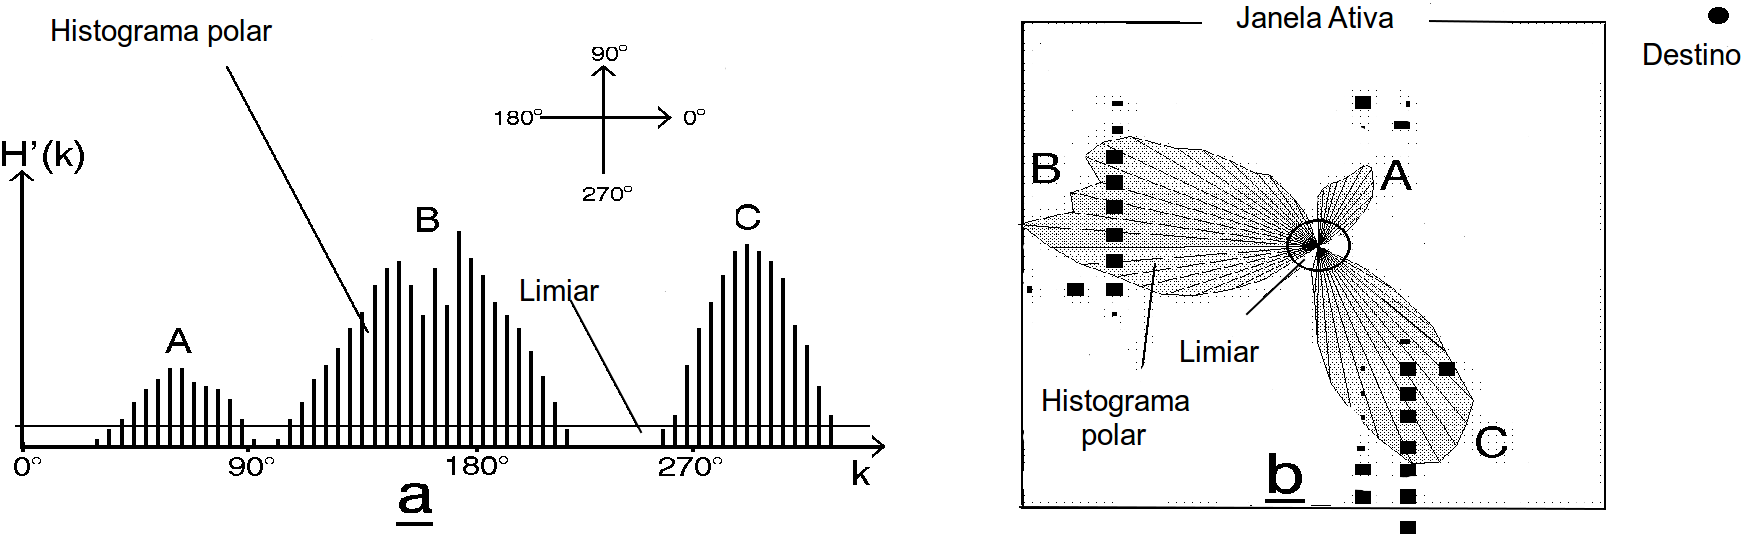
\includegraphics[width=\textwidth,height=7cm]{images/vfh_horiz.png}
	 	\caption{VFH - \textbf{(\underline{a})} Gráfico do histograma, 
	 	onde H'(k) representam as forças de repulsão aos obstáculos nas direções k.\\
	 	\textbf{(\underline{b})} Representação espacial em relação aos 
	 	obstáculos (retângulos em preto) - A área circulada representa a posição do robô.}
		\fonte{adaptado de: \cite{Borenstein1991}}
	 	\label{fig:vfh}
	\end{minipage}
\end{figure}


%Para o planejamento global, de posse de uma mapa convertido em custos 

Enquanto o VFH tem um comportamento mais reativo, em um cenário onde um mapa
global mesmo que incompleto é fornecido pode ser adotado um método deliberativo
para o planejamento da trajetória até um destino.

Os algoritmos de geração de trajetória baseados em amostras tem sido adotado em
robótica móvel com maior ênfase principalmente pela aplicabilidade prática, este
tipo de abordagem leva em consideração a cinemática do veículo gerando
trajetórias realistas com custo computacional baixo \cite{ompl}.

Estes métodos inicialmente constroem um grafo baseado em amostras de trajetórias
que o veículo pode executar, onde geralmente se limita a algumas manobras afim
de reduzir as ramificações do grafo \cite{topologic}. Após esta etapa pode ser
executado um método gráfico de busca por um caminho de menor custo baseado no
menor caminho e proximidade de obstáculos \fig{fig:sbpl}.

\begin{figure}[ht]
	%\hspace{0.1cm}
	\centering
	\begin{minipage}[b]{1\linewidth}
	    \centering
	 	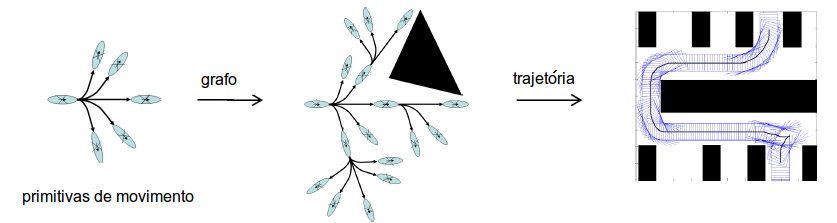
\includegraphics[width=\textwidth,height=5cm]{images/sbpl.png}
	 	\caption{Planejamento de trajetória por amostras}
	 	\fonte{adaptado de: www.ros.org}
	 	\label{fig:sbpl}
	\end{minipage}
\end{figure}
%No trabalho de \cite{} foi utlilizada a biblioteca SBPL
%(\textit{Search-based Planning Library}) 

%Os métodos heurísticos
% baseados em amostra 

\subsection{Controle}

O controle de navegação de um robô móvel pode ser classificado basicamente como
reativo, deliberativo ou híbrido \cite{Wolf2009}, podendo ser estruturada de
forma hierárquica; um caso particular de arquitetura híbrida em camadas. No
projeto COHBRA \cite{Heinen2002}, foi utilizada a abordagem híbrida em camadas
para a criação de um sistema de controle para robôs móveis. Esta abordagem
híbrida permite ao sistema de controle planejar e executar um plano de uma
trajetória (camada deliberativa) ao mesmo tempo em que detecta a presença e
desvia de obstáculos que não foram previamente mapeados (camada reativa). As
técnicas aplicada na elaboração do sistema de controle podem ser baseadas em
Máquinas de Estados Finitos (FSM – \textit{Finite State Machines}), Sistemas
Especialistas e/ou Sistemas Nebulosos (FIS - \textit{Fuzzy Inference Systems}),
Redes Neurais Artificiais (RNA), ou mesmo, uma combinação destes em diversas
camadas. 

As RNAs são consideradas sistemas "caixa-preta": após o treinamento da RNA os
pesos sinápticos associados a cada neurônio (por exemplo, perceptron) não têm
propriamente um “significado”, somente valores numéricos que representam o
conhecimento adquirido. A sua capacidade de generalização torna-a tolerante a
ruídos e permite a aplicação principalmente quando não se consegue estruturar
totalmente o problema a partir de regras bem definidas. É uma técnica
extremamente plástica, podendo ser aplicada a diversas classes de problemas. O
sistema SEVA3D \cite{Heinen2007} se baseou no aprendizado neural de um FSM
(Finite-State Machine) para fazer o controle de navegação do veículo, já no
simulador RoBombeiros \cite{Pessin2008}, adotou-se uma RNA para este fim
(\fig{fig:ann_pesin}).

\vspace{0.5cm}
\begin{figure}[ht]
	%\hspace{0.1cm}
	\centering
	\begin{minipage}[b]{0.6\linewidth}
	    \centering
	 	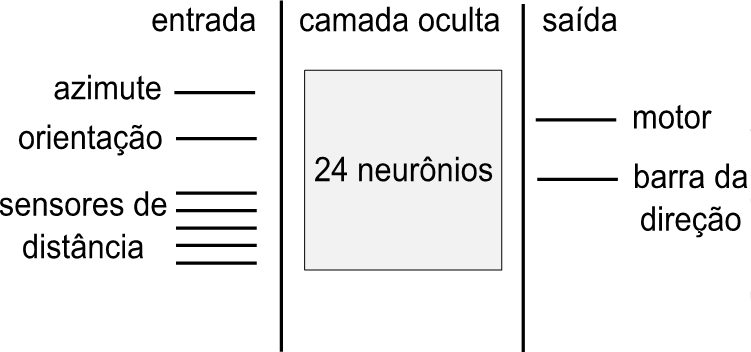
\includegraphics[width=\textwidth,height=5cm]{images/ann_pesin.png}
	 	\caption{Arquitetura da RNA no simulador RoBombeiros}
	 	\label{fig:ann_pesin}
	\end{minipage}
\end{figure}


%OSORIO
%> Podia detalhar um pouco mais sobre o Robombeiros aqui... se não for detalhar
% mais adiante, seria bom ser mais "didático" pois nem todos da banca sabem do
% que se trata e como funciona (assim como os futuros leitores deste texto)

No caso dos RoBombeiros, o controle pela rede neural era de um comportamento
basicamente reativo, onde ao mesmo tempo que direcionava o veículo para o
destino gerava comandos de desvio na presença de obstáculos próximos. Nesta rede
neural foi projetado como entrada a orientação do veículo dada por uma bússola e
a sua orientação em relação ao ponto de destino calculada pelas posições de GPS,
assim como informações sensoriais de distâncias de objetos presentes no raio de
ação do sensor laser utilizado. Desta forma a rede neural foi treinada para
gerar comandos de aceleração e esterçamento que controlavam a navegação do
veículo autônomo.

%2012-10-15 Lido OK

\section{Espaço Tridimensional}

É notório verificar que as abordagens de navegação autônoma de veículos
terrestres mais usuais se baseiam em grande parte na restrição de uma visão
planar do ambiente, ou seja, um mundo plano. De fato, isto simplifica os modelos
e é uma abordagem consciente das suas limitações em relação à fidelidade de
representação do mundo real. Para ambientes controlados e até mesmo problemas
reais restritos a abordagem planar é bem sucedida. Já a abordagem tridimensional
é mais geral do que a abordagem planar pois descreve o espaço em todas as suas
reais dimensões. Portanto, ela contempla o caso planar como caso particular. Por
outro lado, inerentemente o custo computacional associado se torna mais elevado
devido aos aumento da complexidade e dimensionalidade dos modelos.

No que diz respeito a recursos computacionais, a computação embarcada atual já
viabiliza diversas aplicações onde modelos mais completos e complexos se tornam
praticáveis. Isto se traduz não só em maior realismo quando se trata da relação
com o utilizador do sistema como maior precisão devido aos modelos mais
completos. É neste sentido que as abordagens tridimensionais, no que diz
respeito à percepção do ambiente onde se inserem os robôs móveis, têm sido
buscadas pela comunidade científica atualmente.

A visão estéreo se insere neste contexto e é uma ferramenta para a extração da
informação tridimensional do ambiente. Os sensores laser tem desempenhado papel
importante na construção destes algoritmos por produzirem dados precisos a um
baixo custo computacional pois não há a necessidade de transformação do dado
capturado, como ocorre no caso das câmeras. Por outro lado são sensores
extremamente especializados, com características que por vezes limitam sua
aplicação real - são equipamentos sensíveis e geralmente não podem ser cobertos
por uma proteção, por exemplo. Câmeras de vídeo são de uso geral sendo
largamente utilizadas em diversas aplicações.

Conforme descrito na Seção \ref{sec:mapas_disparidade}, a partir de um conjunto
de câmeras através de uma visão estéreo é possível extrair informação visual do
espaço tridimensional do ambiente. Tais dados são convertidos em nuvens de
pontos (\fig{fig:nuvem_pontos}), e assim como para os sensores laser, os métodos
aplicados à interpretação e classificação se dão a partir destes pontos. Uma
nuvem de pontos nada mais é do que um conjunto de pontos no espaço sem
informação de correlação, apenas os dados de pontos no espaço. No caso das
câmeras, a informação cromática pode ainda ser agregada a estes pontos. Em
geral, as nuvens de pontos são classificadas de acordo com a sua densidade,
podendo ser esparsa ou densa. As câmeras apresentam outra vantagem por não só
produzirem pontos tridimensionais como provêem uma imagem do cenário, onde por
métodos de processamento de imagens e de visão computacional é possível extrair
diversas características que permitem uma interpretação da cena não
necessariamente tridimensional.

\vspace{0.5cm}

\begin{figure}[ht]
%	\centering
	\begin{minipage}[b]{0.33\linewidth}
	    \centering
	    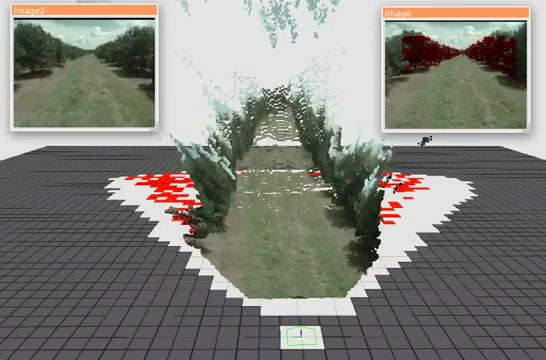
\includegraphics[width=\textwidth,height=4cm]{images/nuvem_pontos_caio.jpg}
	 	\caption{Nuvem de pontos a partir de câmera estéreo}
		\fonte{LRM (divulgação)}
	 	\label{fig:nuvem_pontos}
	\end{minipage}
	\begin{minipage}[b]{0.33\linewidth}
	    \centering
	    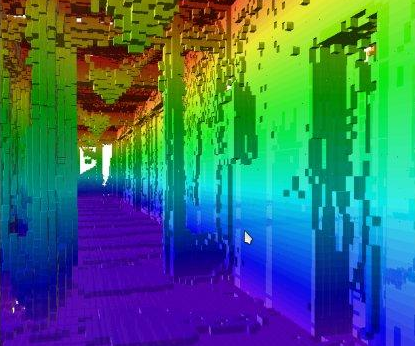
\includegraphics[width=\textwidth,height=4cm]{images/octomap.png}
	 	\caption{Mapa de ocupação (\textit{octomap})}
		\fonte{\\\cite{octomap}}
	 	\label{fig:octomap}
	\end{minipage}
	\begin{minipage}[b]{0.33\linewidth}
	    \centering
	    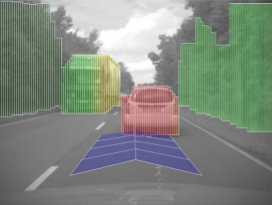
\includegraphics[width=\textwidth,height=4cm]{images/stixel.png}
	 	\caption{Segmentação por \textit{stixels}}
		\fonte{\cite{stixelworld}}
	 	\label{fig:stixel}
	\end{minipage}
\end{figure}

Devido à sua dimensionalidade, a informação a ser tratada é de ordem cúbica
comparada a ordem quadrática no caso planar. Algoritmos eficientes para tratar e
analisar tal volume de dados são necessários. O tratamento da informação deve
ser dado de forma volumétrica levando à necessidade de estruturas de dados
correspondentes. Largamente utilizado em computação gráfica, a representação por
\textit{voxels} é a abordagem tradicional pois permite discretizar o espaço em
sólidos cúbicos, reduzindo assim o espaço de busca. Uma técnica eficiente para a
representação de mapas tridimensionais é apresentada em \cite{octomap} e se
baseia no conceito de \textit{octrees}. Nesta abordagem o espaço é representado
por um \textit{octomap} (\fig{fig:octomap}), de acordo com a ocupação do espaço.
A informação da ocupação do espaço é obtida através de uma nuvem de pontos,
podendo esta ser fornecida de forma incremental, gerando então um mapa do espaço
de forma recursiva.

Outra abordagem de representação da informação tridimensional da cena em
agrupamentos por volumes é apresentada no trabalho de \cite{stixelworld}. Neste
trabalho é introduzido o conceito de \textit{stixel}, que representa um
determinado objeto a partir de sua projeção a partir do solo. O \textit{stixel}
é então um paralelepípedo (\fig{fig:stixel}) que representa uma região ocupada
na cena. Esta abordagem tem sido aplicada em reconhecimento de objetos na cena,
como veículos e pessoas \cite{Benenson2012}. O \textit{stixel} é dado por uma
base retangular e uma altura tendo o plano do chão como origem (representação
também chamada de 2,5 dimensões). Apesar de ser uma representação restritiva do
espaço tridimensional tem se demonstrado vantajosa principalmente em relação ao
seu custo computacional \cite{Benenson2011}.

%OSORIO
%> Ao final de cada capítulo sempre é bom ter uma seção de "Considerações
% Finais", na qual se faz uma reflexão do que foi apresentado (uma visão mais
% ampla de todo conteúdo) e aproveitando para fazer uma relação com o trabalho 
% como um todo e inclusive fazendo um "gancho" para o próximo capítulo

A construção e representação de mapas de ocupação por \textit{octree} se
apresenta mais vantajosa por ser uma representação estruturada dos dados,
enquanto os \textit{stixels} são independentes enquato estrutura de dados.
Porém, para classificação e clusterização de objetos na cena os \textit{stixels} já são
uma representação apropriada. Desta forma, utilizar ambas abordagens vem sendo
estudado com o propósito de agregar ambas características em um mapa de
navegabilidade.


%2012-10-15 Lido parcialmente (pode ser mais desenvolvido)
\section{Considerações Finais}
	
Neste capítulo foram apresentados os principais problemas referentes a navegação
autônoma do veículo relativos às questões de localização, mapeamento e
navegação. Em relação a localização, foi considerada uma proposta de utilização
de sensores do tipo GPS (para a localização) e de uma câmera estéreo (para o
mapeamento local e desvio de obstáculos). Por fim, foram apresentados e feita
uma breve análise sobre métodos de navegação. Baseado nas referências
analisadas, os métodos VFH e RNAs são soluções adequadas para uma navegação
baseada em uma orientação de destino, associada ao desvio de obstáculos
detectados através de uma percepção local. Estes elementos constituem-se
portando dos módulos e componentes deste projeto de pesquisa de mestrado. No
capítulo seguinte será apresentada a metodologia proposta.

%2012-10-14: Lido OK

